\def\year{2018}\relax
%File: formatting-instruction.tex
\documentclass[letterpaper]{article} %DO NOT CHANGE THIS

\usepackage{aaai18}  %Required
\usepackage{times}  %Required
\usepackage{helvet}  %Required
\usepackage{courier}  %Required
\usepackage{url}  %Required
\usepackage{graphicx}  %Required
\frenchspacing  %Required
\setlength{\pdfpagewidth}{8.5in}  %Required
\setlength{\pdfpageheight}{11in}  %Required
\usepackage{subcaption}
\usepackage{todonotes}

\usepackage{amsmath, amssymb, amsthm}
\usepackage[shortlabels,inline]{enumitem}
\usepackage{booktabs}

%\theoremstyle{definition}
\newtheorem{definition}{Definition}

\DeclareMathOperator*{\argmax}{arg\,\!max}
\DeclareMathOperator*{\argmin}{arg\,\!min}

%PDF Info Is Required:
  \pdfinfo{
/Title (Qualitative Discovery of Marine Population Trends)
/Author (Andrea Baisero)}
\setcounter{secnumdepth}{1}  

% The file aaai.sty is the style file for AAAI Press 
% proceedings, working notes, and technical reports.
%
\title{Qualitative Discovery of Marine Population Trends}
\author{Andrea Baisero\thanks{Northeastern University, Boston, USA.}\\\texttt{baisero.a@husky.neu.edu}}

\begin{document}
\maketitle

% \begin{abstract}

% \todo[inline]{Write}

% \end{abstract}

\section{Introduction}

Modern research efforts in the natural sciences (amongst others) are often
driven by a posterior analysis of large multimodal datasets---usually collected
over long periods of time---containing heterogeneous measurements about
a particular domain of interest.  Although a number of main research questions
are necessarily formulated before the whole data collection process can take
place, it is often true that the collected data spans a broader set of
variables (and respective ranges), and that it has a potential to be used for
other purposes which may well be very different from the original intentions
driving the data collection process.  As such, in an effort to be as efficient
as possible in the way that scientists are able to use the available data, it
is very important to develop flexible explorative tools with which an expert
user can probe the data freely and in such a way that he/she has control over
the level of prior context which is being exploited in the visualization.

In this document, we will expose our effort in creating such a tool for
a specific domain---that of marine population analysis---and discuss the design
choices which were made during development.  These will hopefully address
issues and topics which are not only specific to our peculiar domain, but also
of a broader utility within the context of domainless data visualization.

\begin{figure*}
  %
  \centering
  %
  \fbox{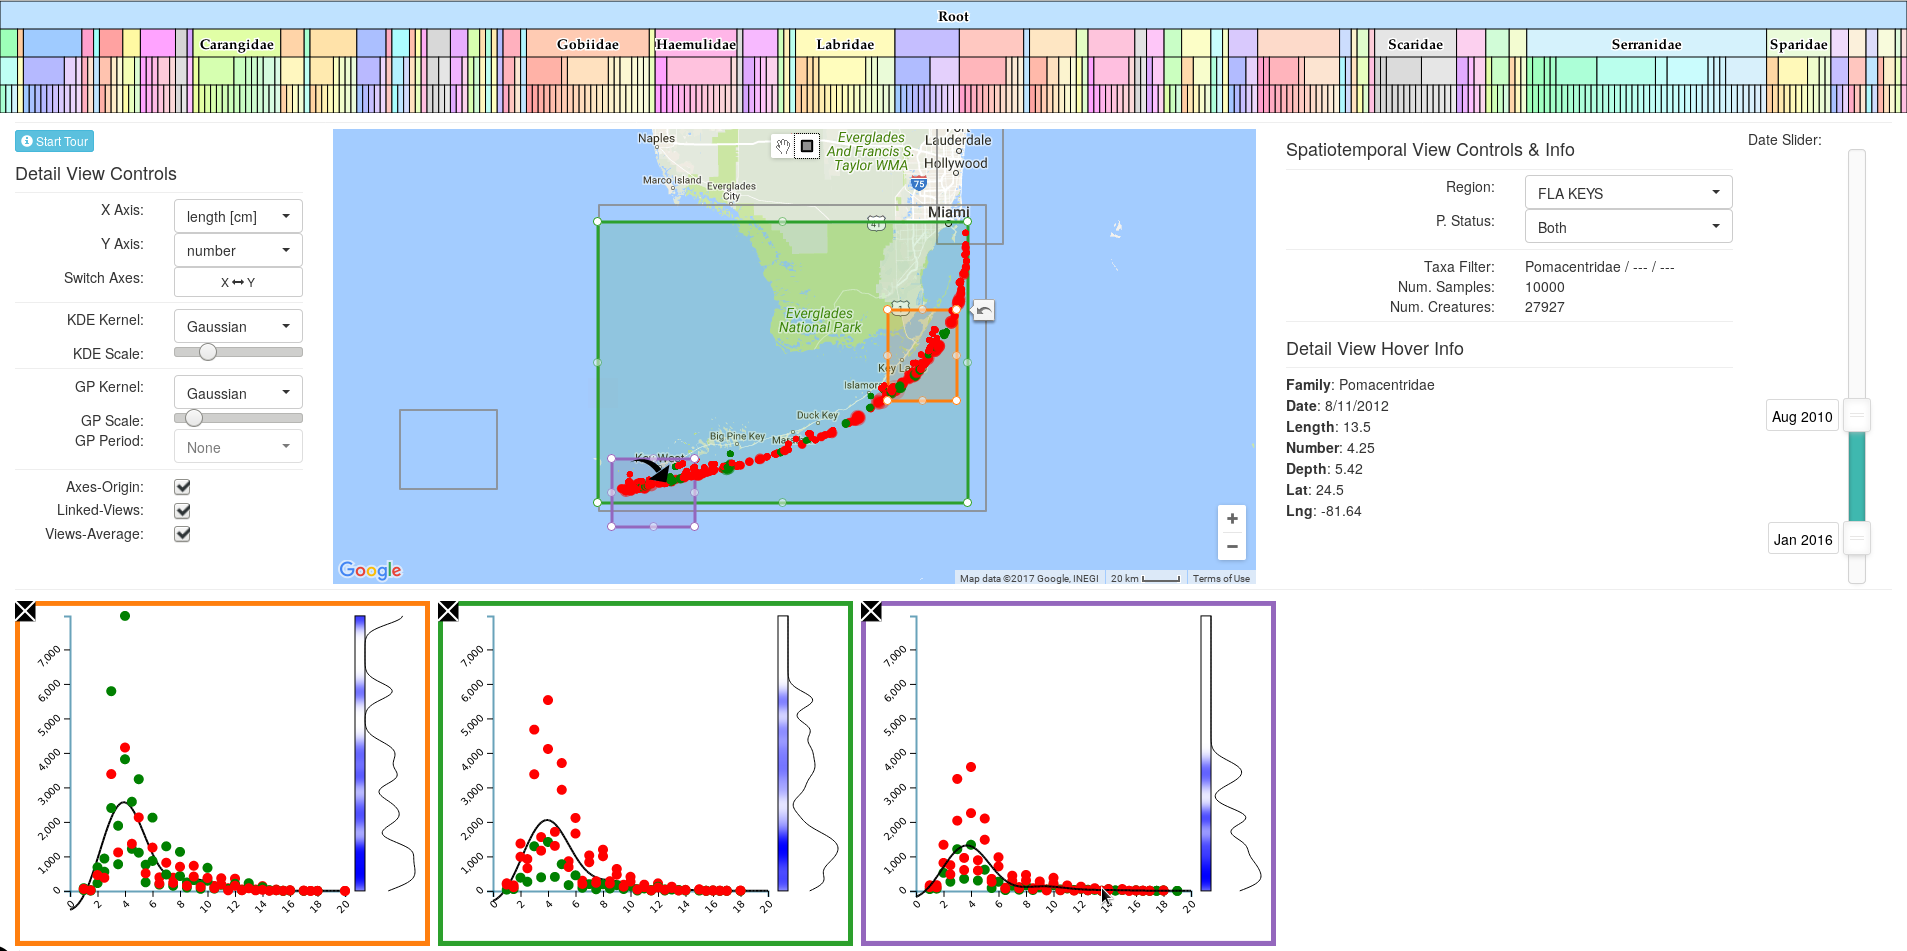
\includegraphics[width=\linewidth]{./figs/screen.png}}
  %
  \caption{Overview of the entire design.  On top, the taxonomy view;  in the
  middle, the spatiotemporal view;  on the right, the spatiotemporal controls;
on the bottom, the detail views;  and on the left, the detail controls.}
  %
  \label{fig:full}
  %
\end{figure*}

\section{Problem Description}

We partnered up with Benjamin
Moran\footnote{\url{https://undergraduate.northeastern.edu/research/profiles/benjamin-moran/}},
a prominent student in Marine Biology who was interested in exploring a dataset
concerning the habitats and populations of aquatic life forms which can be
found in the regions South and South-East of the Florica Bay area during
a temporal window of about 20 years.  We will first describe the components of
the dataset, and then discuss the type of analysis which an user expert in
Marine Biology might want to be able to perform using a tool for qualitative
exploration.

\subsection{Data}

% \begin{figure}
%   %
%   \centering
%   %
%   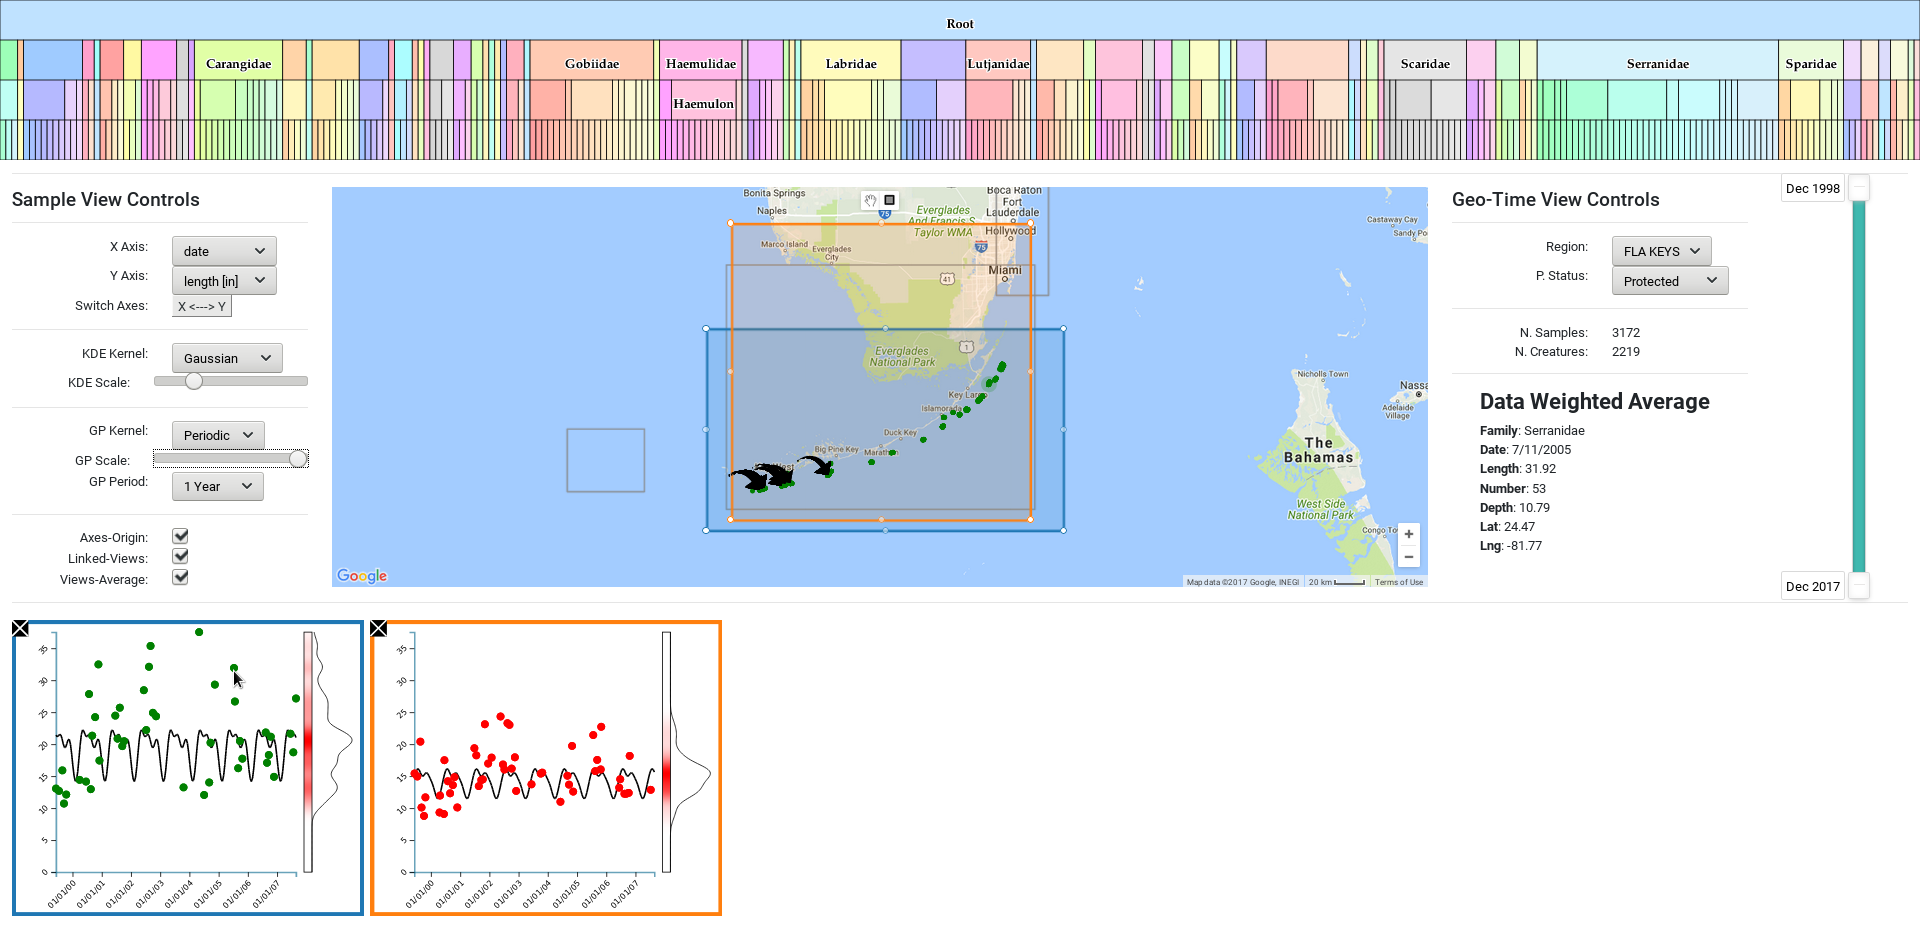
\includegraphics[width=\textwidth]{figs/dviz.png}
%   %
%   \caption{Overview of the design.}
%   %
%   \label{fig:overview}
%   %
% \end{figure}

The data\footnote{Originally available at
  \url{https://grunt.sefsc.noaa.gov/rvc_analysis20/}, although the server has
  been unavailable at certain points even for extended periods of time.
  A secondary access is provided in the form of an R script
\url{https://github.com/jeremiaheb/rvc}, which is however dependent on the
primary server to be active.} is multimodal and partitioned into four
components: \emph{taxonomy} data, \emph{sample} data, \emph{stratum} data, and
\emph{benthic} data.  The number and specificity of fields in each of these
components is very extensive, and we have not incorporated all of them into our
tool;  as such, for the sake of conciseness, we will mainly focus on the fields
which we have used and which are thus more relevant (taxonomy and sample data),
and only give a high-level description of the ones we have not directly used
(stratum and benthic data).

The stratum data contains meta-data about the sampling process, i.e. sampling
locations, dates, protection status, etc.

The benthic data contains information on the ocean floor and coral
reef, the maximum heights of hard and soft reef, percentages of each type of
reef, and amounts of sand, rubble, coral, octocoral and sponge matter.

The taxonomy data describes the biological relationships between different
species.  This is represented as a static hierarchical tree consisting of the
bottom three layers of the standard classification of living organisms in
biological fields, namely \emph{family}, \emph{genus}, and \emph{species}.  For
every species, the minimum length at capture and the median length at maturity
is also specified.

Finally, the sample data represents the heart of the whole dataset, and
describes sample statistics of the collected organisms.  It is essentially
represented a histogram which associates a count to each combination of sample
properties (date, species, depth, size, etc).  Each datum contains a large
number of fields, including underwater visibility, time of sight, habitat type,
etc.  For the sake of simplifying the problem domain, we will only be using
a subset of the available fields, which are the following:
%
\begin{description}
%
  \item[Species Code:]  A code uniquely determining the sample genus and
    species (family is consequently uniquely determined from this information).
    A more common name for the species, which is used in more common speech, is
    also provided;
%
  \item[Region:]  A categorical label indicating one of three regions near the
    Florida Bay area, namely the Florida Keys archipelago (\textit{FLA KEYS}),
    the Dry Tortugas National Park (\textit{DRY TORT}), or the Southeast
    Florida Coral Reef Initiative area (\textit{SEFCRI});
%
  \item[Date:]  The date when the sample was obtained;
%
  \item[Location:]  The latitude and longitude where the sample was obtained;
%
  \item[Protection Status:]  A boolean flag indicating whether the sampling
    location benefits from some form of governmental protection against various
    forms of fishing or pollution;
%
  \item[Depth:]  The distance from the water surface where the sample was
    obtained;
%
  \item[Size:]  The length of the sampled organism; and
%
  \item[Sample Count:]  The number of sampled organisms which match the above
    fields.
%
\end{description}

\subsection{Goal}

The main purpose of our design is that of exploratory analysis with particular
focus on discovering how fish populations and sizes change over time or as
a response to varying environmental factors.  To allow the end user maximum
flexibility on what kinds of relationships to analyze, we will need to provide
both multiple views with the special purpose of \emph{filtering} the data, and
multiple linked views in which the filtered data is to be visualized.  Each
datum contains many heterogeneous subfields, which implies multiple filtering
techniques will be required, e.g. filtering by family, genus and species is
going to differ from filtering by time period which is going to differ from
filtering by region or location.

The success of the design will be measured in terms of what kind of conclusions
can be made using the tool, combined with how flexible the exploration process
itself is.  The evaluation will be performed under the form of two independent
case studies, the details of which are in Section~\ref{sec:evaluation}.

\section{Related Work}

The data we are basing our work on has been collected over the course of
multiple decades, and has been the subject of a number of research efforts The
data sampling process is described in detail in~\cite{smith2011multispecies}.
The document also presents some rudimentary techniques for the visualization of
relevant statistics and geospatial information.  In our work, we hope to
establish more interactive means to explore the same data, albeit with the goal
of obtaining qualitative results which will help the marine biologist to
focalize his own quantitative statistical methods on relevant portions of the
whole data.  De'ath et al.~\cite{de2000classification}, use classification and
regression trees to extract inferential dependence between chosen independent
and dependent variables.  The inferred quantitative dependence is visualized in
the form of the regression tree itself, from which the user is able to see
which independent variables contribute the most, statistically speaking,
towards determining the dependent value.

The data is highly multimodal, and an adequate visualization will necessarily
involve multiple linked views, each of which is focused on a separate aspect of
the data.  To address such a heterogeneous set of visualization needs, the
final design will require the combination of diverse techniques.  Kreft et
al.~\cite{kreft2010framework} address the topic of how to cluster geographical
regions based on species distributions.  Although their evaluation is based on
global-scale regions, their approach could easily be applied to smaller scales
such as that of our domain, the coasts near Southern Florida.  It was our
intention, in our original design, to provide a similar functionality.
However, this idea was finally scrapped due to time constraints in order to
guarantee that more fundamental components were completed.  Rogowitz et
al.~\cite{rogowitz1996not} discuss how different color-schemes impact the
perception of heatmaps with high-frequency and low-frequency variations;  to
avoid the biases involved when using any specific type of heatmap, we will
provide both a heatmap-based view to visualize data density, and one which is
not based on a color-scheme, each of which will serve a different purpose.

Another challenge associated with the visualization of large datasets concerns
the fact that not all the data can be shown at the same time, which fosters the
use of interaction techniques with which the user can navigate the shown data
and select new portions online.  Heer et al ~\cite{heer2012interactive}
describes a thorough taxonomy of interaction techniques, many of which---e.g.
sorting, filtering and selection---will be incorporated in our final design.
Concerning the more specific topic of animation, Heer et
al.~\cite{heer2007animated} outlines a classification of animation techniques
and respective design considerations; We will make sure to guarantee that some
of the more relevant principles are sustained, e.g.  semantic data persistence.
Finally, Liu et al.~\cite{liu2014effects} study the effects of latency in how
a user interacts with an interface, and provide guidelines on how to exploit
such effects not only to improve the user experience, but also on how to
redirect the user's attention towards a proficient direction.  Given the size
of our data, it will be imperative to keep track of the effects of latency; the
positive but especially the negative ones.

\section{Comprehensive Design}

In this section, we go through the three main components of the overall
interface, which we will refer to as the \emph{taxonomy} view, the
\emph{spatiotemporal} view, and the \emph{detail} view.  For each component, we
outline the intended goals that the view needs to satisfy, which difficulties
require particular consideration to achieve such goals, and an aesthetic and
functional description of the chosen design.

\subsection{Taxonomy View}

\subsubsection{Goals and Challenges}

The main usage goal of the taxonomy view is that of allowing the user to
quickly identify and select families/genera/species for data-filtering
purposes.  Despite the taxonomic hierarchy being fairly shallow (with a height
limited by three layers), its large branching factor determines spatial
efficiency as being the main design difficulty which needs to be addressed.  So
in order to achieve the main goal of allowing the user to select elements, we
will need to address and achieve a secondary goal which is that of navigation
through the tree.

\subsubsection{Design}

The original inspiration for the final design derives from the Zoomable
Sunburst~\cite{sunburst}, whose main design objective is that of efficient and
intuitive navigation through subtrees of the hierarchical structure.  This
original design would suffer from a number of issues if it were used for our
application as it stands.  First of all, the angular extension of the original
design is not sufficient to visualize clearly the whole taxonomy tree, except
for excessively big values for the radius.  We address this by flattening the
angular range horizontally, in order to exploit the whole horizontal extension
of the screen;  this also solves the issue of wasted corner space which the
original angular design would imply.  Even after having maximized the space
efficiency, most cells do not have enough space to contain labels indicating
their contents, leaving the user unsure about how to find a specific element.

We address this issue in three alternative complementary ways:  First of all,
we sort each subtree alphabetically, giving the user an intuitive way to
identify the approximate region where to find certain elements even before
interacting with the view.  As a secondary measure, we position a label in each
cell, as long as the label is fully contained within the boundaries (these will
appear and disappear during the navigation process, as the cell sizes change);
Even when the full tree is shown (and, consequently, the fewest labels are
shown), this gives the user an instantaneous and intuitive idea of where to
find cells beginning with specific letters.  Furthermore, during navigation the
cells will become big enough that most cells will be able to contain a label,
thus making the full tree information directly available.  Finally, we add
a tooltip which appears upon hovering each element, to give the user a way to
always have access to full information about a specific cell, independently
from the current navigation state.

The chosen color-scheme was designed to marginally aid the user in
distinguishing between different families, genera, and species at a glance.
Each family is assigned a pastel color with a hue which is unique amongst the
nearby families.  Subsequently, the colors of descendant genera and species are
obtained by applying a small hue variation on the color assigned to the
respective family, as a function of their position relative to the other genera
and species.  This particular choice of color-scheme is perhaps the least
imperative of the design properties of this view, and we can imagine a number
of equally valid alternatives being used.

\begin{figure*}
  %
  \begin{subfigure}[b]{\linewidth}
    %
    \centering
    %
    \resizebox{\hsize}{!}{\fbox{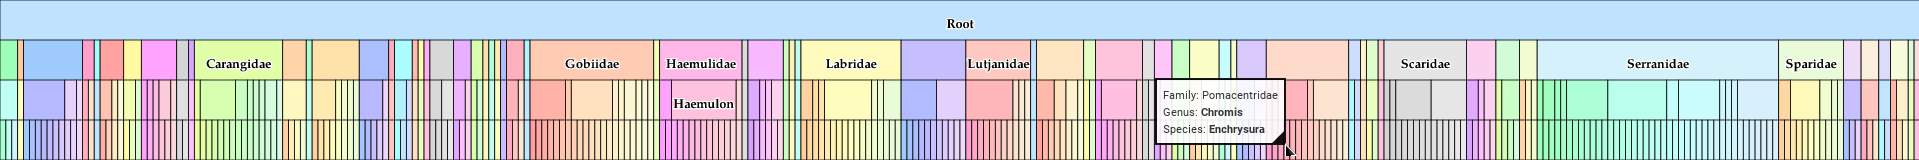
\includegraphics[width=\textwidth]{figs/taxa.png}}}
    %
    \caption{Unexpanded view of the full taxonomy tree.  As shown, labels are
      only visualized for cells which can fully contain them, in order to give
      the user a quick at-a-glance context of where to find cells of interest.
      Further identification of cells is aided by the presence of a tooltip and
    the navigation enabled by the use of a mouse click, as seen in
  \ref{fig:taxa_nav}.}
    %
    \label{fig:taxa_full}
    %
  \end{subfigure}
  %
  \begin{subfigure}[b]{\linewidth}
    %
    \centering
    %
    \resizebox{\hsize}{!}{\fbox{
    %
    \begin{tikzpicture}
      %
      \node (A) at (0,0)
      { 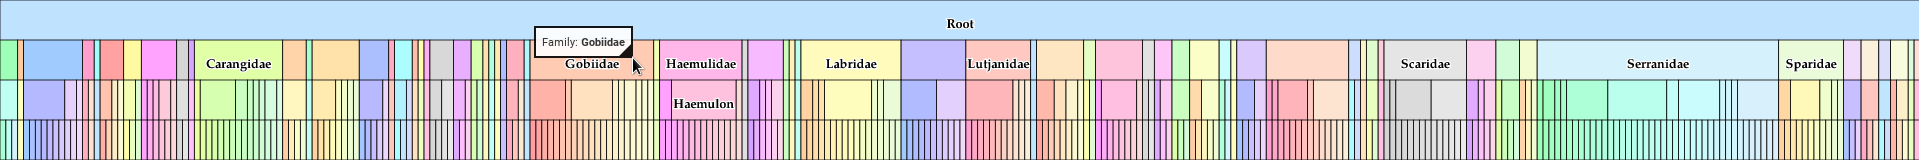
\includegraphics[width=\linewidth]{figs/taxa_click.png} };
      %
      \node (B) at (0,-1.75)
      { 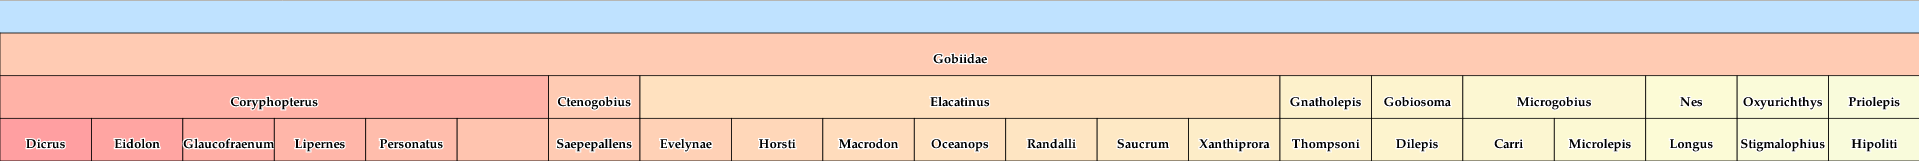
\includegraphics[width=\linewidth]{figs/taxa_expanded.png} };
      %
      \draw[thick] (-2.85, .37) -- (-2.85, -.75) (-2.85, 0) -- (8.9, -1) --
      (8.9, -2.5);
      %
      \draw[thick] (-3.975, .37) -- (-3.975, -.75) (-3.975, 0) -- (-8.9, -1) --
      (-8.9, -2.5);
      %
    \end{tikzpicture}
    %
    }}
    %
    \caption{Expanded view of the \emph{Gobiidae} family branch, as the result
    of a mouse click on the respective family node.  In this case, as in most
  others, the expanded view allows for most labels to be contained within the
respective cells, and thus visible to the user.}
    %
    \label{fig:taxa_nav}
    %
  \end{subfigure}
  %
  \label{fig:taxa}
  %
  \caption{The taxonomy view shows the current state of the taxonomy filter.
  On top, the full taxonomy tree is shown in its original form.  On the bottom,
a sub-tree which was selected by the user during navigation through the
hierarchical structure.}
  %
\end{figure*}

\subsection{Spatiotemporal View}

\subsubsection{Goals and Challenges}

The spatiotemporal view is one of the main references the user has to view and
filter data.  It needs to provide functionalities and means to achieve:
a faithful depiction of the geographic areas and dates under consideration;
controls to manipulate which location- and date-ranges are currently selected
and shown;  visualization of data-points corresponding to the current set of
filters correctly laid on top of the geographic map; and labels indicating
other information which cannot directly be observed from the map view, e.g.
currently taxonomy filter in place, total number of samples and organisms
shown, etc.

\subsubsection{Design}

The spatiotemporal view is split in two panels:  one which contains
a geographic view, and one which contains controls, labels and other space
intended to contain information for the user. 

The geographic view is based on the Google Maps JavaScript API~\cite{gmapsapi},
thus exploiting a number of useful built-in features such as showing an
accurate graphical depiction of the geographic areas of interest, converting
between geographic coordinates and screen pixels, as well as zooming and
panning.  Figure~\ref{fig:geo} shows the three regions of interest, each
outlined by a faint gray rectangle.  An overlay layer is positioned above the
map in order to superimpose graphical information relative to the
concentrations of biological life at the respective coordinates.

Figure~\ref{fig:geo_data} shows the overlay containing data-points relative to
the \emph{Pomacentridae} family.  This view obviously focuses mainly on the
location of each datum, which plays a relatively marginal role when compared to
all the other available fields.  For this reason, this view was designed to
avoid the clutter of information which does not directly relate to the
geographical aspect of each datum (other aspects will be explored in more depth
in the detail views).  More specifically, apart from the actual coordinates, we
encode only one additional aspect of each sample, which is whether the location
benefits from some form of governmental protection status.  Samples in
protected locations are encoded in green, and samples in non-protected
locations are encoded in red.

On the panel to the right, a number of controls are given to the user in order
to further filter the type of data which is shown: A drop-down menu allows the
user to navigate between the three regions of interest, the Florida Keys, the
Dry Tortugas, and the SEFCRI region; a second drop-down menu allows the user to
specify whether to filter samples based on the protection status; and
a vertical slider allows the user to specify a time-range within which the
samples must fall for them to be visualized.  The slider spans a period of
about 20 years at one-month increments.

Furthermore, the panel on the right contains labels indicating the current
state of the taxonomy filter,  how many samples are selected, and how many
individual organisms (which satisfy the prescribed taxonomic, regional,
protection status and date filters) are currently being shown in the geographic
view.  Further empty space is left for use during hover actions in the detail
views, described in the next section.

The geographic view allows the user to draw rectangular areas and create
detail views of the samples contained within these geographic boundaries.
These can be dragged and reshaped later on in order to update the respective
geographic filters online.

\begin{figure}
  %
  \centering
  %
  %\begin{tabular}[b]{cc}
  %  %
    \begin{subfigure}[b]{.4\columnwidth}
      %
      \centering
      %
      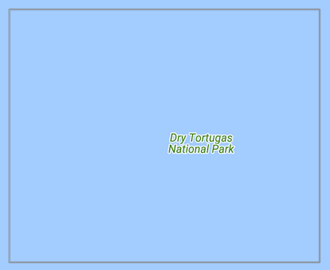
\includegraphics[height=2.75cm]{./figs/DRY_TORT.png}
      %
      \caption{DRY TORT}
      %
      \label{fig:drytort}
      %
    \end{subfigure}
    %
    \begin{subfigure}[b]{.4\columnwidth}
      %
      \centering
      %
      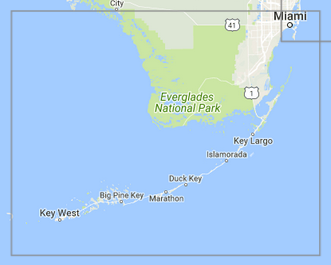
\includegraphics[height=2.75cm]{./figs/FLA_KEYS.png}
      %
      \caption{FLA KEYS}
      %
      \label{fig:flakeys}
      %
    \end{subfigure}
    %
    \begin{subfigure}[b]{.18\columnwidth}
      %
      \centering
      %
      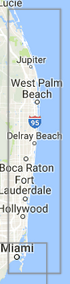
\includegraphics[height=2.75cm]{./figs/SEFCRI.png}
      %
      \caption{SEFCRI}
      %
      \label{fig:sefcri}
      %
    \end{subfigure}
    % %
  % \end{tabular}
  %
  \caption{Geographic views of the Florida Keys, Dry Tortugas and the Southeast
  Florida Coral Reef Initiative (SEFCRI) regions, with superimposed fish-sample
data.}
  %
  \label{fig:geo}
  %
\end{figure}

% \begin{figure}
%   %
%   \centering
%   %
%   \begin{tabular}[b]{cc}
%     %
%     \begin{tabular}[b]{c}
%       %
%       \begin{subfigure}[b]{.5\columnwidth}
%         %
%         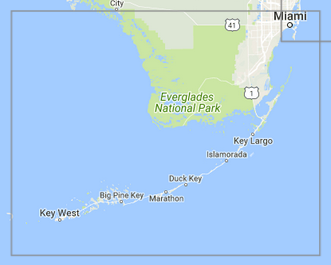
\includegraphics[width=\textwidth]{./figs/FLA_KEYS.png}
%         %
%         \caption{FLA KEYS}
%         %
%         \label{fig:flakeys}
%         %
%       \end{subfigure}
%       %
%       \\
%       %
%       \begin{subfigure}[b]{.5\columnwidth}
%         %
%         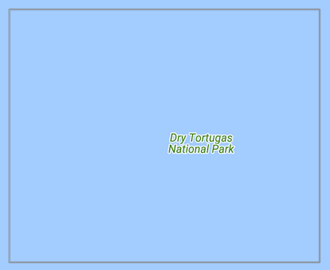
\includegraphics[width=\textwidth]{./figs/DRY_TORT.png}
%         %
%         \caption{DRY TORT}
%         %
%         \label{fig:drytort}
%         %
%       \end{subfigure}
%       %
%     \end{tabular}
%     %
%     \begin{subfigure}[b]{.22\columnwidth}
%       %
%       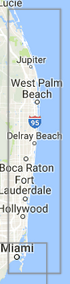
\includegraphics[width=\textwidth]{./figs/SEFCRI.png}
%       %
%       \caption{SEFCRI}
%       %
%       \label{fig:sefcri}
%       %
%     \end{subfigure}
%     %
%   \end{tabular}
%   %
%   \caption{Geographic views of the Florida Keys, Dry Tortugas and the Southeast
%   Florida Coral Reef Initiative (SEFCRI) regions, with superimposed fish-sample
% data.}
%   %
%   \label{fig:geo}
%   %
% \end{figure}

\begin{figure}
  %
  \centering
  %
  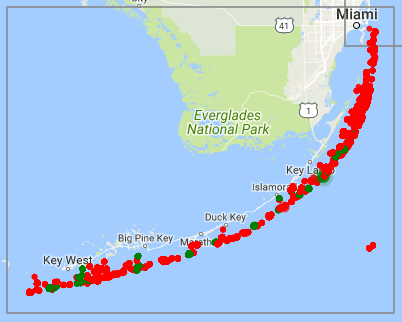
\includegraphics[width=.49\columnwidth]{./figs/geo_pomacentridae.png}
  %
  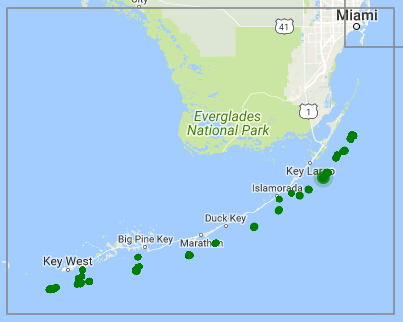
\includegraphics[width=.49\columnwidth]{./figs/geo_pomacentridae_prot.png}
  %
  \caption{Geographic view containing sample data from the \emph{Pomacentridae}
  family.  All the data is shown on the left, while the protection status
filter is applied to the right to show only samples from protected locations.}
  %
  \label{fig:geo_data}
  %
\end{figure}

\subsection{Global and Local Filters}

Before moving on to discussing the detail views, we take a deviation to discuss
how filtering works with respect to those views.  Thus far, we have talked
about various types of filters which the user can manipulate to select which
portion of the data to visualize and analyze, namely filters based on the
taxonomy, geographic region and boundaries, temporal ranges of dates, and
protection status.  Relative to the detail views, each of these filters can be
either \emph{global} or \emph{local}, and either \emph{static} or
\emph{dynamic}.  A global filter is one which applies to all views at the same
time, while a local filter is one which can vary from detail view to detail
view.  Further, a static filter is one which is established at the creation of
a detail view and can not change thereafter, while a dynamic filter is one
which can be changed during the life-span of a detail view.  Next we describe
the properties of each type of filter and, when relevant, the reason for such
decision.

The taxonomy filter is both local and static.  It is local because we want
different views to be able to focus on a different taxonomic element, and it is
static to keep the design simple, given that it is simple enough to create
a new filter for a new species without having to change an older detail view.

The location filters (region and coordinates) are both local and dynamic.  They
are local because we want different views to be able to focus on different
regions, while they are dynamic because we want the user to be able to change
these regions without forcing the creation of a new detail view altogether to
make minor adjustments.

The date filter is global and dynamic.  As opposed to the location filters,
these were chosen to be global because a comparison of different time periods
will be possible anyway by manipulating the detail views themselves, as
described in the next section.  Similarly to the location filters, the date
filter is dynamic to allow the user to change the overall date-ranges of the
shown data-points.

Finally, the protection status filter is both local and static.  It is local in
order to allow the user to better compare statistics relative to one status or
the other.  While we admit that having a dynamic protection status filter may
be a useful feature, we decided to leave it as static in order to simplify the
interface.

\subsection{Detail Views}

The detail views represent the core components of the whole interface.  Each
view represents the most in-depth, detailed and customizable view available to
the user.

\subsubsection{Goals and Challenges}  

These views are inspired by similar flexibility-based efforts such as~\cite{detailtooverview} and~\cite{glostix}.  The main objective in the design
of each detail view is that of giving the user the utmost flexibility in what
data to visualize and how to visualize it.  This means that the user should be
able to choose which data-fields to visualize among the many of available
fields.  Furthermore, the view design should allow the user to analyze not only
the data contained within each view, but also to make valid comparisons across
different views.

\subsubsection{Design}

Figure~\ref{fig:full} shows, on the bottom section, examples of detail views.
Each detail view is associated with a location filter---a rectangle in the
geographic view with the respective color-code---which can be adjusted online.
Each detail view always contains a scatter plot, a one-dimensional heat-map (to
  the right of the scatter plot, and a one-dimensional vertically oriented
  density estimate function (to the right of the heat-map).  Each scatter plot
  shows 3 quantities for each data-point:  two data-fields are shown on the
  respective X and Y axes, while the third is fixed to be the protection status
  of the sample location, encoded as green and red for protected and
  non-protected locations respectively.  Through the use of the available
  controls, shown on the left side of Figure~\ref{fig:full}, the user can
  interact with the detail views and manipulate what is shown and how it is
  shown.  Whenever possible, a transition between configurations is animated in
  order to maintain the data's semantic persistency.

First of all, the data-field associated with the X and Y axes can be changed
through the use of the respective drop-down menus.  On the bottom of the
control panel, three checkboxes allow the user to manipulate the scatter plots.

It is well known that certain graphical representations may introduce a bias if
the axes do not start form the origin.  We allow the user to avoid this
possibility using the \emph{Axis-Origin} checkbox which, when selected, makes
all the axis ranges include the origin, if they don't already and if this makes
sense semantically\footnote{Axes associated with dates and geographic locations
are exempt from this rule.}.

When the default configurations are in place, the ranges of all axes are chosen
to make the data-points span as much space as possible, in order to give the
best possible in-detail view to the user.  Because these ranges are
detail-dependent, comparison across different detail views becomes burdersome,
as the user will need to manually track the corresponding values.  To alleviate
this, the user can use the \emph{Linked-Views} checkbox, which links the axis
ranges of all detail views to be the same.

Further, it is important to remember that the data represents the counts of
a multi-dimensional histogram.  Because the histogram spans multiple
dimensions, there is no single data-point which contains the counts relative to
any given data-field;  rather, these counts are indirectly represented as the
overall counts of many data-points having the same value for that given
data-field.  For example, the counts relative to a specific fish size are split
between the counts relative to that specific size and all depth values, and all
locations, etc.  Continuing with the exmaple, to access the real counts for
a specific fish-size, one needs to aggregate the counts across all other
fields.  This can be achieved by using the \emph{Views-Average} checkbox, which
takes whatever field is selected to be the X-axis, splits its range into
100 bins, and aggregates the data belonging to the same bin together, with the
    sole exception that separate aggregates are computed for protected
    locations and non-protected locations.  If the Y-axis represents the counts
    themselves, then the sum of all aggregated counts is shown;  otherwise
    a weighted average of all values is shown.

Finally, some tentative analysis of the data is provided in the form of two
machine learning methods, kernel density estimation~\cite{bishop2007pattern}
and Gaussian processes regression~\cite{rasmussen2006gaussian}.

Kernel density estimation (KDE) is a method to estimate the relative density of
sample data-points, and in our design it is used to compute the density of
values along the Y-axis\footnote{To view the densities of different
  data-dimensions, the user will have to change what data fielt is associated
with the Y-axis.}.  Each detail view contains two different visualization of
this density: a one-dimensional blue-white heatmap, and a function plot.  The
reason for the double representation is because the heatmap allows for better
comparison of densities across different detail views, while the function plot
allows for better comparison of density values within the same detail view.

Gaussian process regression (GP) is a statistical inference method used to find
regression lines and help the viewer to interpolate the data and generalize
outside of regions with abundance of data-points.  While the method inherently
allows for multi-dimensional regression, we only apply it to plot the Y-axis
data-field regression line against the X-axis data-field.  For the regression
to make sense, it requires the previously described aggregated data, so to
correctly compare the regression line with the scatter plot, the Views-Average
checkbox needs to be activated.  Three types of \emph{kernels}\footnote{A
kernel is a covariance function specifying how information propagates across
different regions in the space of independent variables.} are provided.  The
\emph{Gaussian} kernel implies a convential type of regression, where X-values
which are closer together are more strongly correlated.  On the other hand, the
\emph{periodic} and \emph{locally periodic} kernels---available only when the
date field is chosen as the X-axis---can be used to discover seasonal patterns,
by enforcing high correlations between dates which are distant from each other
as multiple number of times from the selected period.  The periodic kernel is
perfectly periodical, while the locally periodic kernel allows for variations
to appear over long periods of time.  The user can select the period to be
1 month, 3 months, 6 months, or 1 year.


% \begin{figure}
%   %
%   \centering
%   %
%   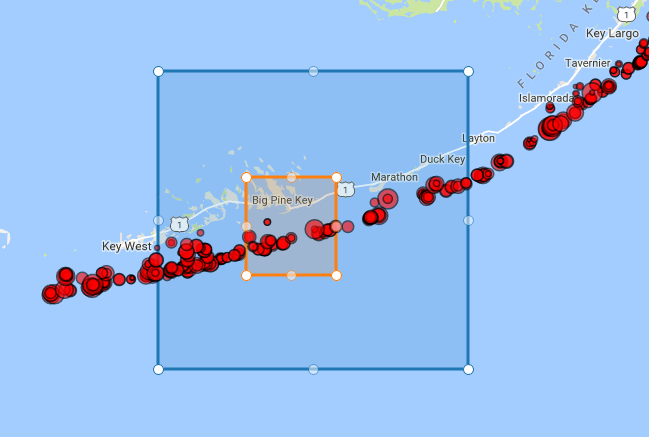
\includegraphics[width=\linewidth]{./figs/filter_rect.png}
%   %
%   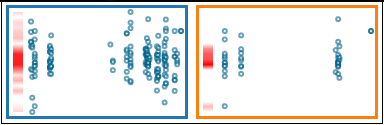
\includegraphics[width=\linewidth]{./figs/filter_plot.png}
%   %
%   \caption{Depiction of two overlapping sample views.  Each selection rectangle
%   establishes a view specific to the samples contained within.  The x-axis
% represents the time when the sample was taken, while the y-axis is the variable
% of interest (e.g. fish length).}
%   %
%   \label{fig:filters}
%   %
% \end{figure}

% \begin{figure}
%   %
%   \centering
%   %
%   \begin{subfigure}[b]{\columnwidth}
%     %
%     \centering
%     %
%     \fbox{
%     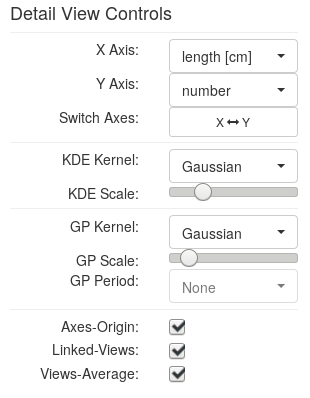
\includegraphics[width=.5\columnwidth]{./figs/detail_ctrls.png}
%     }
%     %
%     \caption{Detail Controls.}
%     %
%     \label{fig:detail_ctrls}
%     %
%   \end{subfigure}
%   %
%   \begin{subfigure}[b]{\columnwidth}
%     %
%     \centering
%     %
%     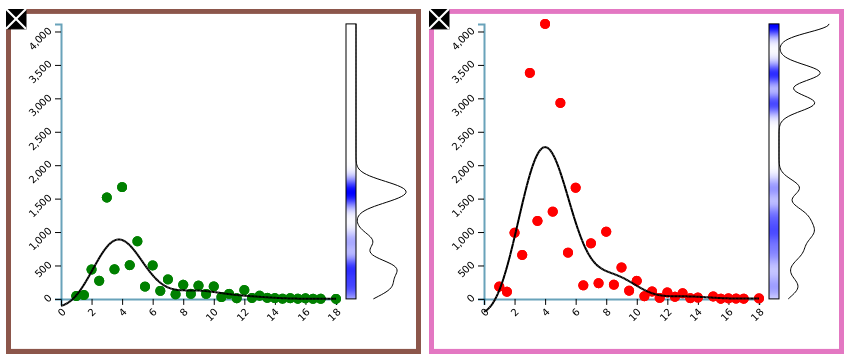
\includegraphics[width=\columnwidth]{./figs/detail_views.png}
%     %
%     \caption{Detail Views.}
%     %
%     \label{fig:detail_views}
%     %
%   \end{subfigure}
%   %
%   \caption{FUCK THIS SHIT.}
%   %
%   \label{fig:details}
%   %
% \end{figure}

% \begin{figure*}
%   %
%   \centering
%   %
%   \fbox{
%   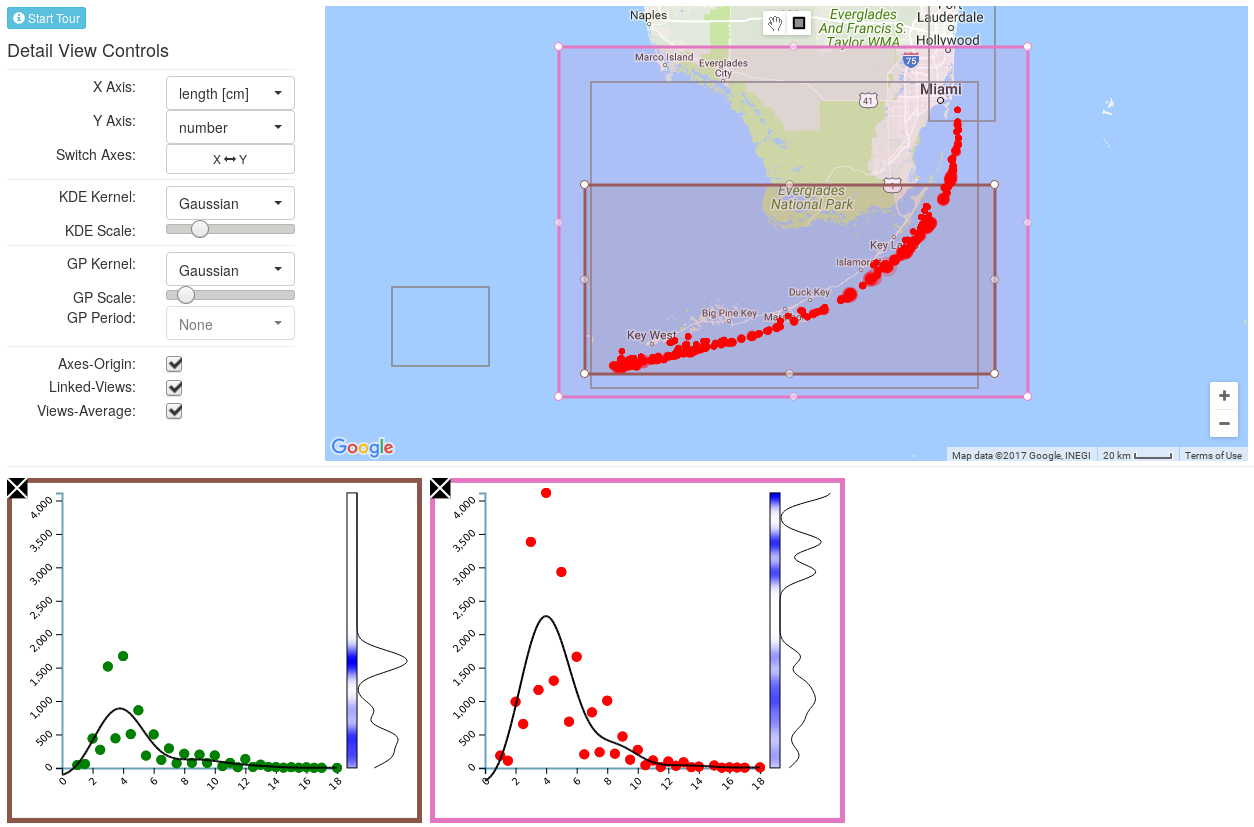
\includegraphics[width=\linewidth]{./figs/detail_views_everything.png}
%   }
%   %
%   \caption{FUCK THIS SHIT.}
%   %
%   \label{fig:details}
%   %
% \end{figure*}

\section{Evaluation} \label{sec:evaluation}

The effectiveness of the design is evaluated through a brief qualitative case
study which demonstrates how to use the visualization tool, and what kind of
findings can be unearthed using it.  More specifically, we wish to explore how
protection status influences the populations and sizes of local fish.  Wanting
large sample sizes to get more accurate results, we decide to select a large
family---the \emph{Serranidae} family---and to adjust the date range such that
it spans the whole 20 years of available data.  Briefly overviewing each of the
three main regions, we find that the Dry Tortugas region has the most distinct
separation between protected and unprotected waters, which is perfect for our
case study objective.

To compare the effects of protection status, we decide to create two detail
view:  For the first one we select ``Protected'' from the protection status
drop-down menu, and then create the selection on the geographic view;  we then
select ``Not Protected'' and create a new selection.

Because the default data-dimensions used in the detail views are the sample
date and sample length, we notice right away that there is a discrepancy
between the sampling dates.  In order to better compare the dates between the
two views, we select the ``Linked-Views'' checkbox.  We now notice two facts:
the first is relative to the sampling process itself, which is that no samples
seem to have been found\footnote{Unfortunately our design provides no clear way
  to distinguish between cases of there merely being no samples found, with
that of there having been no sampling at all.} in the protected areas after
2005;  Secondly, we notice that the protected areas seem to host a larger
quantity of longer samples in the range between 190--240 cm.  To confirm this
last observation, we change the X-axis from ``date'' to ``number'', switch the
axes, and then check the ``Views-Average'' checkbox.  What we obtain is
a histogram of lengths, and we can easily notice that the distribution of
lengths in the protected status areas has both a highest peak (which is to be
expected, given that it spans a larger area), and a longer tail.

\section{Conclusions}

Although some of the original design objectives have been achieved, the tool as
a whole suffers from a number of issues which would require substantial further
effort to fix and mend.

For example, the whole interface incurs in extreme lagging when too many
data-points are selected, e.g. when selecting data from a large family, while
using the whole 20-year range of available dates.  To alleviate this
artificially, a cap has been put on the server such that it can only
serve\footnote{I do not have the details regarding the order in which the
data-points are server, and thus on whether there is any inherent bias in how
these are selected.} a maximum of 5000 samples.  Obviously this is not an
adequate solution to the problem, and a better one should be found.  Further,
the detail views only offer limited capability, both in terms of data and axis
manipulation, and in terms of automatic analysis which is available (KDE and
GP).

\subsection*{Who Did What}

This project started as a collaboration between me (Andrea Baisero) and Ryan
Cebulko, which later broke off into two separate projects\footnote{I am still
lacking an explanation as to why this happened.}.  In this section, I outline
who took care of completing which aspects of the project before the project
split.  In chronological order, also accounting for all individual components
of the project schedule and requirements:

\begin{description}
  %
  \item[Initial Ideas:] Equal effort and work.
  %
  \item[Critique:] I did not complete this assignment, Ryan did (I'm not sure
    if this assignment is also considered group-work or not, I did not believe
  so at the time).
  %
  \item[Partner/Status Update:] Equal effort and work.
  %
  \item[Proposal:] Mostly completed by me, with Ryan making minor adjustments
    before posting.
  %
  \item[Designs:] Almost exclusively completed by me, with Ryan providing
    a single picture for me to include post-deadline.
  %
  \item[Usability:] Equal effort and work.
  %
  \item[Drafts:] Completed by me alone.
  %
  \item[Presentations and Paper \& Material:]  The group was split after the
    drafts deadline, so I worked on my own as part of a single-person group for
    the remaining deadlines.
  %
\end{description}

Concerning the actual project material, this is what was developed by whom:

\begin{itemize}
  %
  \item I wrote a script to download all the data from the original server
    (originally split into multiple files) and aggregate it into a smaller set
    of CSV files.
  %
  \item Ryan wrote a script to create a database and load the data into it, an
    (incomplete) program to locally serve the data from the database, and used
    a third-party library to create the date slider.
  %
  \item I wrote and designed every other aspect of the actual
    interface\footnote{The tour is based on a third-party
    library~\cite{bootstraptour}, the map on Google Maps~\cite{gmapsapi}, while
  all other visualization components are written in d3~\cite{d3}.}:  the overall
  layout, the taxonomy view, the geographic view, the detail views, the tour,
  the ML algorithms, and all other controls and functionalities.  Many of these
  were completed (or partially completed) before the group split.
  %
\end{itemize}

{\footnotesize
\bibliographystyle{aaai}
\bibliography{cit}
}

\end{document}
